\documentclass[a4paper]{article}

\usepackage[T5]{fontenc}
\usepackage[utf8]{inputenc}
\usepackage{amsfonts,amssymb}
\usepackage{mathtools}
\usepackage[iso]{datetime}
\usepackage{tabu}
\usepackage[colorlinks=true,urlcolor=blue,linkcolor=black]{hyperref}
\usepackage{tkz-graph}
\usepackage{listings}

\title{Advanced Algorithms\\\large Lecture 9}
\date{2017-01-08 \\ Last edited \currenttime\ \today}
\author{Lecture by Shay Mozes\\Typeset by Steven Karas}

\DeclarePairedDelimiter\abs{\lvert}{\rvert}

\newenvironment{itemize*}%
  {\begin{itemize}%
    \setlength{\itemsep}{0pt}%
    \setlength{\parsep}{0pt}%
    \setlength{\parskip}{0pt}}%
  {\end{itemize}}

\newenvironment{enumerate*}%
  {\begin{enumerate}%
    \setlength{\itemsep}{0.5pt}%
    \setlength{\parsep}{0pt}%
    \setlength{\parskip}{0pt}}%
  {\end{enumerate}}

\begin{document}

\maketitle

\section{Agenda}
\begin{enumerate*}
  \item Linear Programming wrapup
  \item Randomized Algorithms
\end{enumerate*}

\section{Linear Programming}

\subsection{Standard Form}
Maximize $\sum\limits_{j=1}^n c_j x_j$ subject to $\begin{matrix}\sum_{j=1}^n a_{ij} x_j & i=1 ... m \\ x_j\ge 0 & j = 1 ... n\end{matrix}$.

\paragraph{Standard matrix form:}
Maximize $C^\intercal x$ such that $Ax \le b$ and $x \ge 0$.

\subsection{Integer Programming}
Introduces an additional constraint that $x_j \in \mathbb{N}$. Note that this type of problem is NP-Hard.

\subsection{Branch and Bound}
Algorithm for solving IP problems.

\paragraph{Examples}

\begin{itemize*}
  \item \href{http://optlab-server.sce.carleton.ca/POAnimations2007/MILP.html}{Interactive example}
  \item \href{http://optlab-server.sce.carleton.ca/POAnimations2007/BranchAndBound.html}{Scheduling example}
\end{itemize*}

\paragraph{Example: Weighted Vertex Cover}
Given a graph $G=(V,E)$ with non-negative weights $w(v)$ on the vertices.
Find a minimum-cost set of vertices $S$ such that all the edges are covered.
An edge is covered iff at least one of its endpoints is in $S$.

Reminder: Vertex cover is NP-Complete. The best known approximation factor is $2-\left( \frac{\log \log |V|}{2 \log |V|} \right)$

Let the variables be $x(v)$ for $v\in V$ as whether $v$ is in the cover or not.
Minimize $\sum_{v\in V} w(v) \times (v)$ such that $x(v) + x(u) \ge 1 \;\, \forall (u,v) \in E$ and $x(v) \in \{0,1\} \; \forall v\in V$.

\subsection{Linear Relaxation}
BIP is difficult to solve, so we relax the constraint that $x_j \in \mathbb{N}$ to $0 \le x_j \le 1$. Note that sometimes, we can easily extend the relaxation to $x_j \ge 0$, if the objective function is such that it always helps.

\paragraph{Example: Weighted Vertex Cover as Relaxed Linear Program}
Given a graph $G=(V,E)$ with non-negative weights $w(v)$ on the vertices.
Find a minimum-cost set of vertices $S$ such that all the edges are covered.
An edge is covered iff at least one of its endpoints is in $S$.

Let the variables be $x(v)$ for $v\in V$ as whether $v$ is in the cover or not.
Minimize $\sum_{v\in V} w(v) \times (v)$ such that $x(v) + x(u) \ge 1 \;\, \forall (u,v) \in E$ and $x(v) \ge 0 \; \forall v\in V$.

\paragraph{Example: WVC}\ \\
\begin{figure}[h!]
\centering
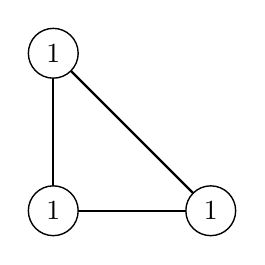
\begin{tikzpicture}
  \SetGraphUnit{2}
  \Vertex[L=$1$]{A}
  \EA[L=$1$](A){B}
  \NO[L=$1$](A){C}
  \Edge(A)(B)
  \Edge(B)(C)
  \Edge(C)(A)
\end{tikzpicture}
\end{figure}

Optimizing this gives us an invalid solution of $1/2$ for each vertex. 

This strategy can give us an invalid solution, but if we can prove an approximation to the optimal solution, we can get an easy way to approximate NP-Hard problems.

\[SOL \le 2 \cdot OPT_{LP}\]
\[OPT_{LP} \le OPT_{VC}\]


\paragraph{2-approximation for WVC}
First, solve the LP-Relaxation. Let $S$ be the set of all the vertices $v$ with $x(v) \ge 1/2$. Output S as a solution.

Now we will prove that this is a 2-approximation to weighted vertex cover:
The solution is feasible: for each edge $e=(u,v)$,
either $x(v) \ge 1/2$ or $x(u) \ge 1/2$
In our solution we've increased $x(v)$ by a factor of at most 2 (turned $x(v)=1/2$ to $1$). Hence the cost of the solution is at most $2\cdot OPT_{LP}$
Since $OPT_{LP} \le OPT_{VC}$, the cost of the solution is $\le 2 \cdot OPT_{VC}$.

\subsection{LP Duality}
Consider LP: $\max c^{\intercal}x$ such that $Ax \le b$, $x \ge 0$.
$n$ variables, $m$ constraints.

How large can the optimum $c^\intercal x$ be?

Consider a vector $y$ of $m$ variables.
If we demand that $y \ge 0$ then $y^\intercal Ax \le y^\intercal b$.
If we demand that $c^\intercal \le y^\intercal A$ then $c^\intercal x \le y^\intercal Ax$.

So $c^\intercal x \le y^\intercal Ax \le y^\intercal b$.
How small can $y^\intercal b$ be?

Minimize $b^\intercal y$ such that $A^\intercal y \ge c$, $y \ge 0$.
This is called the dual LP.

\paragraph{Alternative definition:}
Primal problem: maximize $c^\intercal x$ such that $Ax \le b$, $x \ge 0$.
Dual problem: minimize $b^\intercal y$ such that $A^\intercal y$, $y \ge 0$.

In the primal problem, $c$ is the cost function and $b$ was in the constraint. In the dual problem, their roles are swapped.

Inequality signs are flipped and the maximization turned into minimization. For each constraint in the primal, there is a variable in the dual. For every variable in the primal, there is a constraint in the dual.

\paragraph{Intuition}
The maximization problem produces a solution that is at most as good as the minimization problem, and the converse.

\paragraph{Example:}
Maximize $4p+q+2r$ such that $p + 2q + r \le 2$, $2p+5q-3r \le 3$ and $p,q,r \ge 0$.

\[c^\intercal= \begin{bmatrix}4 & 1 & 2\end{bmatrix}\]
\[A=\begin{bmatrix}1 & 2 & 1 \\ 2 & 5 & -3\end{bmatrix} \begin{bmatrix}p \\ q \\ r\end{bmatrix} \le \underbrace{\begin{bmatrix}2 \\ 3\end{bmatrix}}_{b}\]
\[A^\intercal=\begin{bmatrix}1 & 2 \\ 2 & 5 \\ 1 & -3\end{bmatrix} \begin{bmatrix}x \\ y\end{bmatrix} \le \underbrace{\begin{bmatrix}4 \\ 1 \\ 2\end{bmatrix}}_{b}\]

See slide 64 for a table that describes the general form of duality.

\paragraph{The Duality Theorem}
Let $P, D$ be an LP and its dual.
If one has an optimal solution then so does the other, and their values are the same.

\paragraph{Example: Diet Problem}
As a poor student, we want to spend as little money as possible on food. However, we need to also eat enough to stay alive and healthy.

In a proper diet, we need to eat 4 units of protein a day. Peanut butter provides 1 unit, and costs 2\$. Steak provides 2 units, and costs 3\$.

Let $x=$ the amount of peanut butter per day in the diet.
Let $y=$ the amount of steak per day in the diet.

So we want to minimize $2x+3y$ subject to the constaints $x+2y \ge 4$, $x \ge 0$, and $y \ge 0$.

\subparagraph{Dual problem:}
Maximize $4p$ such that $p \le 2$, $2p \le 3$, and $p \ge 0$.
In this case, $p$ represents the marginal cost per unit of protein.

Intuitively, we can think of these as supply and demand problems, wherein the dual of the diet problem is the supply problem that informs a synthetic protein manufacturer how much they can raise prices to compete with peanut butter and steak.

\paragraph{Practicality}
Sometimes the dual problem will be quicker/easier to solve for some algorithms.
Can be used to bound how far your current solution is from the optimum.
The interplay between the primal and its dual can be used in designing algorithms.

\paragraph{Max flow and it's dual}
the max flow and min-cut problems are duals. More details can be found on slides 68-70\footnote{We did not cover this because we're a little behind this year}.

\subsection{Complementary Slackness}
Primal problem: maximize $c^\intercal x$ such that $Ax \le b$, $x \ge 0$ yields $y^\intercal Ax \le y^\intercal b$.
Dual problem: minimize $b^\intercal y$ such that $A^\intercal y$, $y \ge 0$ yields $x^\intercal A^\intercal y \ge x^\intercal c $.

Recall that $b^\intercal y \le y^\intercal Ax \le c^\intercal x$.
For optimial solutions, $b^\intercal y^*=c^\intercal x^*$ and therefore $b^\intercal y^* = y^{*^\intercal} Ax^* = c^\intercal x^*$.

$(y^{*^\intercal}A - c^\intercal)x^* = 0$ iff $\forall j$ either $x_j^*=0$ or $\sum_{i=1}^m A_{ij} \cdot y^*_i = c_j$.
$y^{*^\intercal}(b-Ax^*)=0$ iff $\forall i$ either $y^*_i=0$ or $\sum_{j=1}^n A_{ij} \cdot x^*_j = b_i$

\paragraph{WVC}
Minimize $\sum_{v\in V} w_v \cdot x_v$ such that $x_v+x_u \ge 1 \;\; \forall (u,v) \in E$ and $x_v \ge 0 \; \forall v \in V$.
The dual of this is to maximize $\sum 1 \cdot y_e$ such that $\sum_{e=uv \in E} 1\cdot y_e \le w_v \; \forall v \in V$ and $y_e \ge 0 \; \forall e \in E$.

By solving the relaxed dual problem, we can quickly cut down the problem size:

\[x_v = \begin{cases}
1 & \text{if }\sum_{(uv) \in E} y^*_{uv}=w_v \\
0 & \text{else}
\end{cases}\]

There is a full formal proof of optimality on slides 75-76.

\[\sum_{v\in V}w_vx_v \le \sum_{v \in V} \sum_{(u,v) \in E} y^*_{uv}=2 \sum_{(u,v) \in E} y^*_{uv} = 2 \cdot OPT_{LP} \le 2 \cdot OPT\]

\paragraph{Idea:}
LPs model many important practical problems. Solving an LP is often an important component of solving or approximating the solution to an IP problem.

We can solve these in polytime, and the simplex algo works fairly well in practice.

NOTE: Use libraries/packages here. NIH hurts like hell.

\section{Randomized Algorithms}

Recommended reading: Randomized Algorithms by Rajeev Motwani and Prabhakar Raghavan.

Random algorithms use a PRNG. Its behavior is defined both by its input and its PRNG. It is often impossible to predict the output of the algorithm. Non-deterministic.

\paragraph{Why?}
\begin{itemize*}
  \item Efficiency
  \item Simplicity
  \item Avoiding the impact of bad cases
  \item Fighting an adversary
\end{itemize*}

\paragraph{Las Vegas algorithms}
Answers are always correct, but the running time is random.
When analyzing these, we attempt to bound expected running time.

\paragraph{Monte Carlo algorithms}
Running time is fixed, but the answers may be incorrect.
When analyzing these, we attempt to bound the error probabilities.

\subsection{Entropy Sources}
Random numbers are collected from entropy sources such as physical phenomena, user's mouse movements, etc.
Mostly, we use pseudo-random number generators (PRNGs), which take a few "good" random bits and generate a lot of "fake" random bits.

\subsection{Agenda}
\begin{enumerate*}
  \item Approximating $\pi$
  \item Selection problem
  \item Randomized data structure
  \item Analysis of random walk on a graph
  \item Randomized graph algorithm
  \item Primality testing
\end{enumerate*}

\subsection{Probability Theory Recap}

Let the sample space $\Omega$ be the set of possible outcome points.
An event is $A \subseteq \Omega$ be a subset of outcomes.
$Pr(A)$ is the probability of an event:
for every event $A$: $Pr(A) \in [0, 1]$
If $A \cap B = \varnothing$ then $Pr(A \cup B) = Pr(A) + Pr(B)$.

This continues on, but isn't really worth it for me to continue, so just look at it on slides 10-12.

\subsection{Markov's Inequality}
If $X$ is a non-negative random variable with expectation $E[X]$ then $Pr[X > 2 E[X]] \le 1/2$.
\footnote{A full algebraic proof can be found on slide 16}

\[\forall a > 0 : Pr[X > a] \le E[X] / a\]

\subsection{Example: Approximating \texorpdfstring{$\pi$}{pi}}
\begin{lstlisting}[frame=L]
findPi(points):
  in_circle = 0
  points times:
    x = random in [0, 1]
    y = random in [0, 1]
    if (x,y) inside circle:
      in_circle += 1

  return (4 * in_circle) / points
\end{lstlisting}

How many points must we use to get an accuracy of $\delta=0.01$?

Let $X_i=1$ iff the $i^{\text{th}}$ point is in the circle.
$E[X_i]=Pr[X_i=1]=\pi / 4$, which implies that $E[X_1 + ... + X_n]=E[X_1] + ... + E[X_n] = n \pi / 4$.
Let $X=\sum X_i$. Our accuracy is is the distance of $4X / n$ from $\pi = 4 E[X] / n$.
We want to bound $Pr[|4X/n - \pi| > \delta]$.

Using Markov's Inequality, we get that:

\[Pr\left[\frac{4}{n} X - \pi > \delta \right] = Pr\left[X > \frac{n(\delta + \pi)}{4}\right] \le \frac{E[X]}{\frac{n(\delta+\pi)}{4}} = \frac{\pi}{\delta + \pi}\]

\subsection{Chernoff-Hoeffding Bound}
Used to bound the convergence of sums of random variables $X=X_1+...+X_n$.
Let $X_i$ be indicator variables ($X_i \in \{0, 1\}$).
All the variables must be independent: $\forall i \ne j: Pr[X_i=1|X_j=1] = Pr[X_i=1]$
Let $\mu = E[X] / n$.

When satisfied, the sum converges exponentially fast:

\[Pr\left[ \abs*{\frac{X}{n}-\mu} \ge \delta \right] \le 2e^{-\frac{n\delta^2}{3\mu}}\]

Using this\footnote{I wasn't paying attention, but there was an algebraic derivation of this on the whiteboard}, we can bound the error in our $\pi$ approximation example to:

\[\varepsilon=0.05, \delta=0.01 \Rightarrow n > \frac{3\pi \ln 40}{4 \cdot 0.0001} \approx 86917\]


\end{document}
